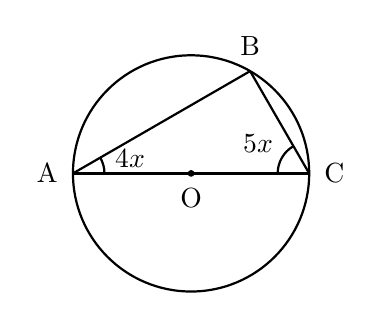
\begin{tikzpicture}[scale=1]

    % Define the center of the circle
    \coordinate (O) at (0,0);

    % Draw the circle
    \draw[thick] (O) circle (1.5);

    % Define points on the circle
    \coordinate (A) at (180:1.5);
    \coordinate (B) at (60:1.5);
    \coordinate (C) at (0:1.5);

    % Draw the lines and segments
    \draw[thick] (A) -- (C);
    \draw[thick] (A) -- (B);
    \draw[thick] (B) -- (C);

    % Draw the angle arcs
    % Arc at A (between AC at 0 degrees and AB at 30 degrees)
    \draw[thick] (A) ++(0:0.4) arc (0:30:0.4);
    
    % Arc at C (between CA at 180 degrees and CB at 120 degrees)
    \draw[thick] (C) ++(180:0.4) arc (180:120:0.4);

    % Add labels for the points
    \node[left, xshift=-2pt] at (A) {A};
    \node[above, yshift=2pt] at (B) {B};
    \node[right, xshift=2pt] at (C) {C};
    \node[below, yshift=-2pt] at (O) {O};
    
    % Add a small dot for O
    \filldraw (O) circle (1pt);

    % Add angle values inside the arcs using relative positioning
    \path (A) ++(15:0.75) node {$4x$};
    \path (C) ++(150:0.75) node {$5x$};

\end{tikzpicture}